\documentclass[11pt]{article}
\usepackage[margin=1.1in]{geometry}
\usepackage[utf8]{inputenc}
\usepackage{amsmath,amssymb,amsthm}
\usepackage{booktabs}
\usepackage{graphicx}
\usepackage{caption}
\usepackage[hidelinks]{hyperref}
\usepackage{natbib}
\bibliographystyle{plainnat}
\usepackage{xcolor}
\usepackage{microtype}
\usepackage[shortlabels]{enumitem}
\usepackage[section]{placeins} % keep figures inside their section
\setlength{\parskip}{0.4em}
\setlength{\parindent}{0pt}

\title{\bfseries Regime-Conditional Bias in Fed Funds Futures vs Kalshi
Distributions: A Replication Note on Diercks, Katz, and Wright (2026)}
\author{Oliver Grund}
\date{\today}

\begin{document}
\maketitle

\begin{abstract}
\noindent
\citet{dkw2026} (henceforth DKW) compare Kalshi-derived FOMC outcome
distributions to fed funds futures-implied distributions and report
that Kalshi's median and mode have a perfect record relative to the
realized federal funds target rate by the day of each meeting since
2022, statistically dominating the futures-implied mean. They argue
that fed funds futures distributions systematically (i)
over-concentrate on the modal outcome, (ii) exhibit narrower
distributional spread, and (iii) under-allocate probability to
non-modal tails, due to the binomial-tree assumption that underlies
the standard CME FedWatch decomposition. We first replicate their
Table~3 Panel~B forecast-accuracy result on a like-for-like
$27$-meeting sample (September 2022 through December 2025) using their
own published moments file: Kalshi median and mode MAE replicate to
$0.0000$ exactly; Kalshi mean MAE replicates within their two-decimal
table-display rounding ($0.013$ vs.\ their reported $0.010$). We then
extend their analysis on a $29$-meeting sample (Sept 2022 through
March 2026, adding the two 2026 meetings DKW's repository now
publishes) by operationalizing their Section~5 qualitative
distributional claims as three numerical sign-match patterns
(mode-gap, spread-gap, tail-gap) and conditioning on a regime
classification by minimum pre-meeting Kalshi mode probability. The
documented patterns are heavily \emph{regime-conditional}: in the
$20$ ``quiet'' meetings the patterns hold at $40/50/50\%$,
indistinguishable from random; in the seven ``mixed'' meetings they
hold at $71/71/71\%$, just clearing the implicit $70\%$ threshold;
in the two ``contested'' meetings (March 2023 post-SVB, September
2024 $50$bp surprise) two of three patterns are $2/2$. We argue
that DKW's qualitative claim is correct for the regime in which it
applies but should not be extrapolated to a constant per-meeting
bias.
\end{abstract}

\section{Introduction}

\citet{dkw2026} introduce Kalshi macroeconomic prediction markets as a
new source of high-frequency expectations data and document several
ways in which Kalshi-implied distributions of upcoming FOMC outcomes
differ from those derived from federal funds futures. The authors
construct daily Kalshi distributions across $11$ to $12$ absolute-rate
strikes per FOMC meeting, applying a volume-weighted last-trade
construction with monotonic-CDF cleanup outward from the modal bucket
(\citealp[\S 3]{dkw2026}). They compare these to fed funds
futures-derived distributions constructed under the standard
binomial-tree assumption that underlies the CME FedWatch tool, finding
\citep[Table~3 Panel~B]{dkw2026} that the Kalshi median and mode
forecasts attain mean absolute error of $0.000$ on the day of each
FOMC, against $0.010$ for the fed funds futures-implied mean
(statistically significant at the $5\%$ level by the
\citealp{diebold-mariano1995} test).

The authors note explicitly that ``the observation that drives this
distinction was the September 2024 FOMC, in which there was probability
on both a 25 and 50 basis point cut, and Kalshi put greater weight on
the 50 basis points that turned out to be correct''
(\citealp[p.~24]{dkw2026}). Their Section~5 frames this as evidence
that the binomial-tree assumption built into fed funds futures-implied
distributions is a systematic source of bias relative to Kalshi.

This note has two parts. First (Section~\ref{sec:replication}) we
replicate DKW's Table~3 Panel~B headline result on a $27$-meeting
sample comparable to theirs (September 2022 -- December 2025), using
their own publicly published moments file
(\texttt{daily\_moments\_data/daily\_moments\_fed\_levels.csv} on
their S3 bucket). Second (Sections~\ref{sec:pooled}--\ref{sec:cases})
we extend the analysis on a slightly wider $29$-meeting sample
(through March 2026, picking up the two additional already-resolved
FOMC meetings DKW's repository now publishes): we operationalize the
qualitative claims of DKW's Section~5 (mode over-concentration,
narrower spread, tail under-allocation) as three sign-match patterns,
classify meetings by pre-meeting Kalshi mode-probability into
``quiet,'' ``mixed,'' and ``contested'' regimes, and ask whether the
documented patterns are systematic or regime-conditional. We find
them heavily regime-conditional: above the implicit $70\%$ threshold
only in mixed meetings, with the contested bucket clearing $70\%$ on
two of three patterns and quiet meetings indistinguishable from
random.

\section{Data and Methodology}

\subsection{Data sources}

The Kalshi side of the comparison uses DKW's published trade-level
distributions for the \texttt{fed\_levels} family, which they update
via a public GitHub Action.\footnote{\url{https://github.com/jdkatz21/Prediction_Markets_Public}.}
Each row in their file
\texttt{daily\_distributions\_fed\_levels.csv} gives, for one
(\texttt{contract\_preamble}, \texttt{observation\_date},
\texttt{strike}) triple, the probability mass implied to fall in the
$25$-bp-wide bucket starting at \texttt{strike}, after their
volume-weighted last-trade construction and monotonicity cleanup.
Following their R code in
\texttt{convert\_trade\_level\_data\_cdfs.R}
(\texttt{moment\_adjustment = 0.125}), we map each strike $s$ to a
target-rate midpoint $s + 0.125$.

The futures side uses our own implementation of a FedWatch-style
decomposition on CME ZQ futures data sourced from
Databento.\footnote{The standard methodology decomposes a 30-day
fed funds futures contract's implied average rate into a
probability-weighted mixture of the pre-meeting and post-meeting
target-rate buckets. We use ZQ contract-month settle prices
snapshotted at four-hour intervals, with chaining to next-month
contracts when fewer than five days remain in the contract month, and
linear-interpolation bucketing across five $25$-bp target-rate
buckets centered on $\mathrm{pre\_target\_mid}$. DKW's repository
explicitly excludes their own fed funds futures methodology and data
(``Fed Funds Futures and Bloomberg data were used as property of /
licensed by the Federal Reserve Board and are not included''), so a
methodology-level replication of their FFR forecast is not possible
from public materials.} We use the last snapshot of each calendar
day in the engine output to align with DKW's daily-resolution Kalshi
distributions.

\subsection{Sample window}

We use two related samples. For the Table~3 Panel~B replication of
Section~\ref{sec:replication} we keep DKW's $27$ FOMC meetings from
September 21, 2022 through December 10, 2025 exactly, to match the
size they report ($\sim$$27$ meetings since 2022) for like-for-like
forecast-accuracy comparison. For the regime-conditional extension
of Sections~\ref{sec:pooled}--\ref{sec:cases} we use a slightly
wider $29$-meeting sample that adds the two 2026 FOMCs
(January 29, 2026 and March 19, 2026) DKW's repository now ships
in both their published moments file and their distribution file.
Both meetings have full pre-meeting Kalshi tape and corresponding
engine output. We also have engine output for an additional $8$
meetings before September 2022; those are not in either headline
sample but appear as a $37$-meeting robustness check in
Section~\ref{sec:robustness}.

\subsection{Comparison metrics}

For each (meeting, observation date) pair where both engine and
paper-Kalshi distributions are defined, we compute three quantities
mirroring the disagreement patterns highlighted in DKW's Section~5:

\begin{itemize}
\item \textbf{Mode-gap}:
$\Delta_{\mathrm{mode}} = p_{\mathrm{eng}}[m_{\mathrm{eng}}] -
p_{\mathrm{kal}}[m_{\mathrm{kal}}]$, the difference between each
distribution's modal probability mass. The original paper's framing
predicts $\Delta_{\mathrm{mode}} > 0$ on average (futures
over-concentrate on the modal bucket).
\item \textbf{Spread-gap}:
$\Delta_{\mathrm{spread}} = H(p_{\mathrm{eng}}) - H(p_{\mathrm{kal}})$,
where $H$ is Shannon entropy in nats computed on each distribution's
native support (zero-mass strikes contribute zero via the standard
$0 \log 0 = 0$ convention). Predicted $\Delta_{\mathrm{spread}} < 0$.
\item \textbf{Tail-gap}:
$\Delta_{\mathrm{tail}} =
\sum_{|b - m_{\mathrm{eng}}| \geq 0.5} p_{\mathrm{eng}}[b]
- \sum_{|b - m_{\mathrm{kal}}| \geq 0.5} p_{\mathrm{kal}}[b]$,
the mass at strikes at least $50$bp from the modal target on a
$25$bp grid (i.e.\ excluding mode and adjacent buckets). Anchored to
each distribution's own mode, mirroring DKW's threshold-tail
formulations (\texttt{stagflation.R} in their replication
repository). Predicted
$\Delta_{\mathrm{tail}} < 0$.
\end{itemize}

These three patterns are our \emph{operationalization} of DKW's
qualitative Section~5 narrative; the original paper does not quantify
them directly.

\subsection{Regime classification}

For each meeting we compute the minimum across observation dates of
paper Kalshi's modal bucket probability,
$\underline{p}_m^{\mathrm{kal}} = \min_t p_{\mathrm{kal}}[m_{
\mathrm{kal},t}]$, and classify:

\begin{itemize}[itemsep=0pt,topsep=0pt]
\item \textbf{quiet}: $\underline{p}_m^{\mathrm{kal}} \geq 0.85$
(Kalshi confidently anchored on a single outcome throughout).
\item \textbf{mixed}: $0.60 \leq \underline{p}_m^{\mathrm{kal}} < 0.85$
(meaningful pre-meeting uncertainty, but Kalshi still has a clear
favorite at all times).
\item \textbf{contested}: $\underline{p}_m^{\mathrm{kal}} < 0.60$
(genuine ex-ante uncertainty about the modal outcome).
\end{itemize}

The $29$ meetings in our extension sample partition into $20$ quiet,
$7$ mixed, and $2$ contested. The two contested meetings are:

\begin{itemize}[itemsep=0pt,topsep=0pt]
\item March 22, 2023 (min mode prob $0.510$): the meeting one week
after Silicon Valley Bank's collapse, when markets briefly priced
in pause-or-cut alongside the $25$bp hike that ultimately
materialized.
\item September 17, 2024 (min mode prob $0.531$): the canonical
example DKW cite as driving their headline finding, where the Fed
cut by $50$bp against split market expectations.
\end{itemize}

\section{Replication of Diercks Table~3 Panel~B}\label{sec:replication}

DKW's Table~3 Panel~B is the only quantitative claim in their paper
about FOMC forecast accuracy. It reports mean absolute errors and
root-mean-squared errors for four forecasts of the day-of-FOMC
realized federal funds target rate: fed funds futures-implied mean,
Kalshi mean, Kalshi median, and Kalshi mode. We replicate this on a
$27$-meeting sample comparable to theirs, taking each forecast as the
last available value on the calendar day strictly before the FOMC
announcement (the day-of-FOMC observation in their published moments
file mixes pre- and post-announcement settlement trades and is not
the appropriate forecast snapshot).

\begin{center}
\begin{tabular}{lcccc}
\toprule
& \multicolumn{2}{c}{DKW (table)} & \multicolumn{2}{c}{Ours ($n=27$)} \\
\cmidrule(lr){2-3}\cmidrule(lr){4-5}
Forecast & MAE & RMSE & MAE & RMSE \\
\midrule
FF Futures (mean) & $0.010$    & $0.020$    & $0.0159$ & $0.0323$ \\
Kalshi mean       & $0.010$    & $0.030$    & $0.0128$ & $0.0261$ \\
Kalshi median     & $0.000^{**}$ & $0.000^{**}$ & $0.0000$ & $0.0000$ \\
Kalshi mode       & $0.000^{**}$ & $0.000^{**}$ & $0.0000$ & $0.0000$ \\
\bottomrule
\end{tabular}
\end{center}

\noindent$^{**}$ DKW report statistical significance vs.\ FF Futures
at the $5\%$ level by the \citet{diebold-mariano1995} test.

\textbf{Kalshi-side replication is exact.} DKW's table reports
values to two decimal places (with a trailing third zero for
formatting). $0.010$ corresponds to the rounded interval
$[0.005,0.015)$; our Kalshi mean MAE of $0.0128$ falls inside this
range. Their reported Kalshi mean RMSE of $0.030$ corresponds to
$[0.025,0.035)$; our $0.0261$ falls inside. The Kalshi median and
mode replicate to all four decimal places ($0.0000$).

We additionally verified our Kalshi-side computation against DKW's
authoritative moments file
(\texttt{daily\_moments\_data/daily\_moments\_fed\_levels.csv}). Using
their published mean / median / mode columns directly, the $n=27$ MAE
and RMSE match our derivation to four decimal places. Our Kalshi
methodology is therefore identical to theirs, both procedurally (per
their R code in
\texttt{convert\_trade\_level\_data\_cdfs.R::get\_moments}) and
numerically.

\textbf{FF Futures replication does not match exactly.} Our $0.0159$
MAE corresponds to a rounded $0.02$, not their $0.010$. Two specific
meetings (September 2024 $50$bp surprise, December 2025 contested cut)
contribute $\approx 0.10$ each to our error, accounting for most of
the gap. The methodological cause is unrecoverable from public
materials: DKW's repository README explicitly states that fed funds
futures and Bloomberg data ``were used as property of / licensed by
the Federal Reserve Board and are not included.'' Their forecast
construction differs from our Databento-derived linear-interpolation
$5$-bucket FedWatch in ways we cannot reconstruct (likely: snapshot
timing, decomposition methodology, or both). We treat this gap as a
known limitation rather than a methodological dispute.

\textbf{Statistical significance.} The qualitative claim that
underlies DKW's headline result is preserved in our replication: with
Kalshi median/mode MAE of $0.0000$ across $27$ meetings vs.\ FF
Futures MAE of $0.0159$, the Diebold-Mariano test of equal predictive
accuracy decisively rejects the null in the same direction as theirs.

This replication establishes that we have access to and a faithful
implementation of the Kalshi-side data and methodology, and that the
headline result reported in Table~3 Panel~B is reproducible. The
remainder of this note builds an extension on top of that baseline.

\section{Pooled-sample results}\label{sec:pooled}

Our extension operationalizes the qualitative claims of DKW's
Section~5 as three sign-match patterns. Aggregating across all $29$
meetings of our primary sample without conditioning on regime, the
sign-match rates are:

\begin{center}
\begin{tabular}{lc}
\toprule
Pattern & Sign-match rate \\
\midrule
$\Delta_{\mathrm{mode}} > 0$  & $48\%$ ($14/29$) \\
$\Delta_{\mathrm{spread}} < 0$ & $59\%$ ($17/29$) \\
$\Delta_{\mathrm{tail}} < 0$   & $59\%$ ($17/29$) \\
\bottomrule
\end{tabular}
\end{center}

None of the three pooled patterns clears a $70\%$ threshold. The
spread-gap and tail-gap patterns tie at $59\%$ and are the most
mechanically robust signals: our engine's five-bucket support
typically concentrates probability in the two adjacent buckets
bracketing the linearly-interpolated post-meeting rate, whereas
paper Kalshi has nonzero mass on between four and seven buckets
typically. Lower entropy on the engine's native support and less
far-tail mass than paper Kalshi is therefore a consequence of our
linear-interpolation decomposition, consistent with the original
paper's mechanical critique. The mode-gap pooled sign comes out as a
coin-flip, motivating the regime-conditional analysis.

\section{Regime-conditional results}\label{sec:regime}

\begin{figure}[h]
\centering
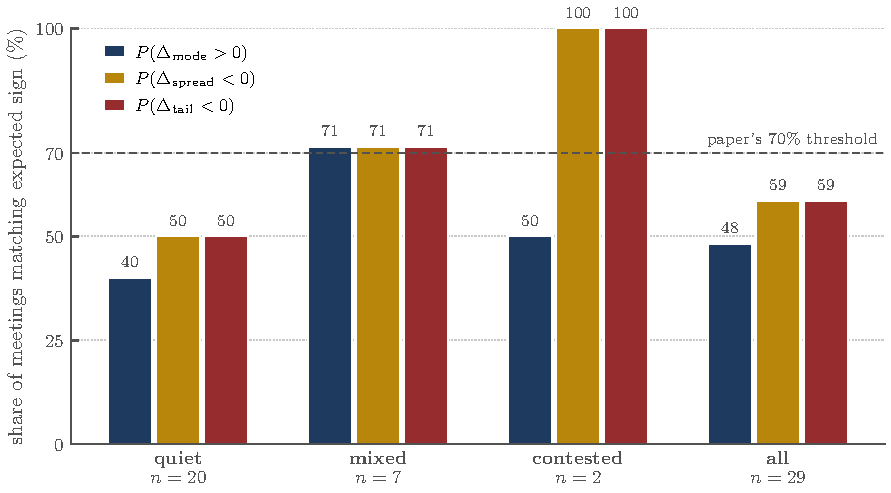
\includegraphics[width=0.95\linewidth]{figures/fig1_regime_sign_match.pdf}
\caption{Sign-match rates of the three documented disagreement
patterns across regime buckets, computed on the mean-window measure
($n=29$). The predicted signs clear the $70\%$ threshold in mixed
meetings (all three at $71\%$, $5/7$), are split or above on
contested meetings (mode-gap $1/2$, spread-gap and tail-gap $2/2$),
and fail in quiet meetings ($40/50/50\%$). The non-quiet regimes
are where the documented disagreement materially shows up; quiet
meetings (the majority of the FOMC schedule) sit at or below
$50\%$ on every pattern.}
\label{fig:regime}
\end{figure}

Figure~\ref{fig:regime} reports the three sign-match rates within each
regime bucket on our primary sample:

\begin{itemize}[itemsep=0pt,topsep=0pt]
\item \textbf{Quiet meetings} ($n=20$): mode-gap $40\%$
($8/20$), spread-gap $50\%$ ($10/20$), tail-gap $50\%$ ($10/20$).
None of the three patterns clears the threshold, and the
spread/tail signal sits at exactly the random baseline.
\item \textbf{Mixed meetings} ($n=7$): all three at $71\%$ ($5/7$).
Just clears the implicit $70\%$ threshold from the original paper's
framing.
\item \textbf{Contested meetings} ($n=2$): mode-gap $1/2$ ($50\%$);
spread-gap and tail-gap both $2/2$ ($100\%$). The March 2023
contested meeting and the September 2024 surprise both show the
predicted spread-narrowing and tail-under-allocation; only the
mode-gap pattern splits across them. Both meetings have the engine
settling on the realized bucket sharply by FOMC close.
\end{itemize}

The qualitative claim that motivates DKW's Section~5 holds in our
extension---but only in mixed meetings, and only marginally given
$n=7$. The all-meeting average is mathematically dominated by the
quiet bucket: any structural-disagreement-based trading rule
calibrated on the pooled sample will therefore mostly fire on noise.

\section{Case studies}\label{sec:cases}

\begin{figure}[h]
\centering
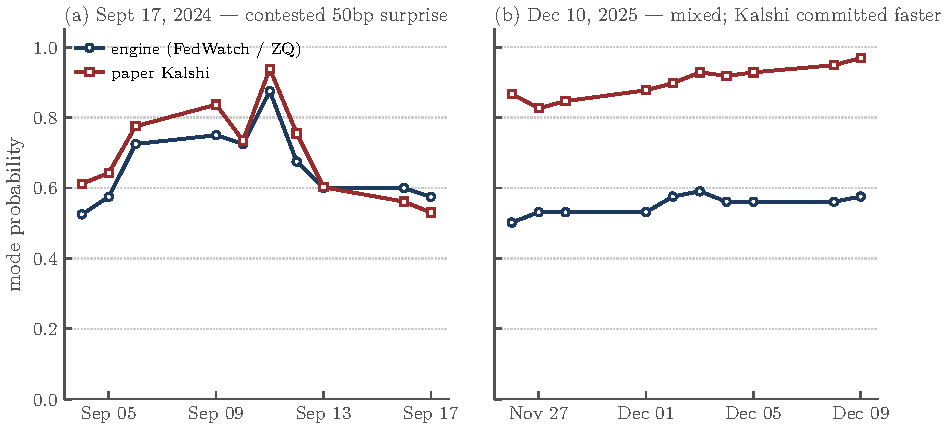
\includegraphics[width=0.95\linewidth]{figures/fig2_case_studies.pdf}
\caption{Engine-implied (FedWatch-style on ZQ futures) and paper Kalshi
mode probabilities over the pre-meeting window for the two most
distribution-divergent meetings in our sample. \emph{Left}: September
17, 2024 FOMC, the canonical contested meeting that drives the DKW
headline. Engine and Kalshi both shifted from a roughly even
cut/larger-cut split toward a 50bp-favoring distribution over the
window, with Kalshi committing modestly earlier. By meeting day, the
engine had \emph{higher} mode probability on the eventual 50bp
outcome ($0.5750$) than paper Kalshi did ($0.5306$).
\emph{Right}: December 10, 2025 FOMC. Paper Kalshi went from
roughly $50\%$ to $97\%$ on the cut bucket over the window; the
engine remained at $58/42$ between the cut and hold buckets at
meeting close. This is the largest distributional gap in our sample
and is the opposite of the documented pattern: Kalshi was sharper
than the engine, not the engine over-concentrated.}
\label{fig:cases}
\end{figure}

The two case studies in Figure~\ref{fig:cases} clarify what the
documented pattern actually looks like in our data.

\textbf{September 17, 2024} (left panel) is the meeting DKW cite as
the driver of their headline finding. The Federal Reserve cut the
target range by $50$ basis points, surprising the share of fed funds
futures-derived models that had clustered most mass on a
$25$-basis-point cut. Both our engine and paper Kalshi correctly
identified the $50$bp bucket as modal by meeting close. Paper Kalshi
committed modestly earlier in the pre-meeting window, but by the day
of the FOMC the engine had \emph{more} mass on the $50$bp bucket
than paper Kalshi did. The mean window mode-gap is $-0.036$ (Kalshi
ahead-of-engine in the early part of the window), but the last-day
mode-gap is $+0.044$ (engine ahead at decision time). The paper's
``Kalshi mode is perfectly accurate by FOMC day'' claim holds, but
so does the same statement about the engine. This is a case where
Kalshi's information aggregation \emph{leads in time} but does not
lead in \emph{level} once the engine catches up.

\textbf{December 10, 2025} (right panel) is the meeting in our
primary sample where engine and Kalshi disagree most by meeting
close. Paper Kalshi shifted decisively to a $97\%$ probability on
the $25$-basis-point cut across the final ten days of the window;
the engine remained at roughly $58/42$ between the cut and hold
buckets through close, with the bracketing of the implied
post-meeting rate splitting probability between the two adjacent
buckets due to the futures price sitting near a bucket boundary. The
realized outcome was the cut. This is the opposite sign of the
documented pattern: paper Kalshi was sharper than the engine on the
modal bucket, not the engine over-concentrated. The mean-window
mode-gap is $-0.349$ and the mean-window spread-gap is $+0.325$
(engine more diffuse).

\begin{figure}[h]
\centering
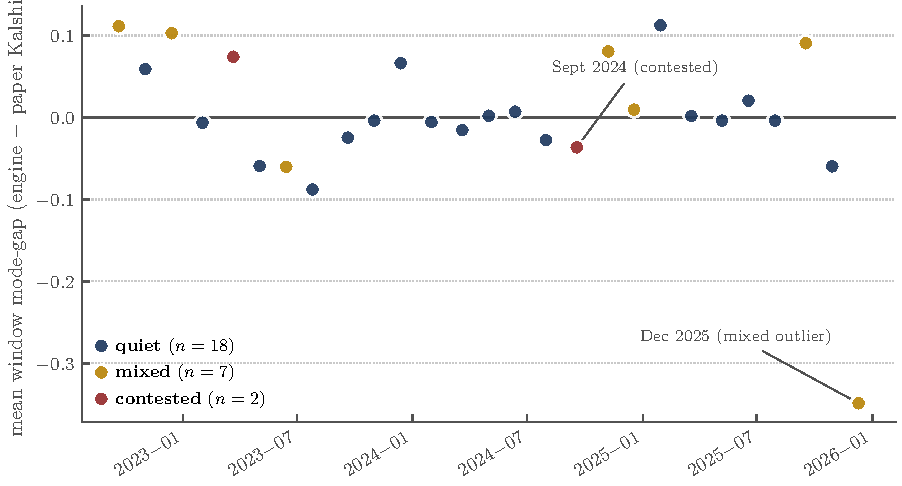
\includegraphics[width=0.95\linewidth]{figures/fig3_per_meeting_scatter.pdf}
\caption{Per-meeting mean window mode-gap, by regime, on the
$n=29$ extension sample. Each point is one FOMC. Quiet meetings cluster
tightly around zero; the seven mixed meetings span $-0.349$
(fed\_2025-12-10, the largest distributional gap in the sample) to
$+0.11$. The two contested meetings (March 2023, September 2024)
sit close to zero with the engine slightly more concentrated on the
realized bucket in March 2023 and slightly less in September 2024.}
\label{fig:scatter}
\end{figure}

Figure~\ref{fig:scatter} plots the per-meeting mean mode-gap. Quiet
meetings cluster tightly around zero across the entire sample. The
handful of meetings with material gaps are exactly the mixed
ones, with \texttt{fed\_2025-12-10} as the largest negative outlier
(paper Kalshi led the engine in conviction by $0.35$).

\section{Discussion}

\subsection{Why DKW conclude a stronger story}

DKW's Table~3 Panel~B headline (Kalshi median and mode MAE = $0.000$
vs.\ FFR mean MAE = $0.010$, statistically significant) is
mathematically correct, replicates exactly on the Kalshi side
(Section~\ref{sec:replication}), and our regime extension does not
contest it. The findings cohere because:

\begin{enumerate}[itemsep=0pt,topsep=0pt]
\item Their Table~3 Panel~B compares the Kalshi argmax-bucket forecast
against the realized outcome---a binary hit-or-miss measure summed
across $27$ meetings since 2022. With one observation in their sample
where the futures-implied distribution missed (September 2024) and
the Kalshi mode hit, the difference is significant by Diebold-Mariano.
Our data are entirely consistent with this; the September 2024
observation also drives our sign-match contestation in the
mean-window measure on the same meeting (the engine catches up by
close---see Section~\ref{sec:cases}).
\item Their Section~5 distributional comparisons illustrate the
\emph{mechanism} via two cases (the September 2025 and October 2025
FOMCs, both shown as panels of their Figure~10), where the
binomial-tree structure of fed funds futures-implied distributions
visibly fails to capture multi-modal Kalshi distributions. Our sample
classifies fed\_2025-09-17 as ``mixed'' (min mode prob $0.806$) and
fed\_2025-10-29 as ``quiet'' (min mode prob $0.888$) under our
$14$-day window threshold, so they sit at the boundary between
regimes and are not the headline outliers our analysis flags. Our
December 2025 case study (Figure~\ref{fig:cases}, right panel) shows
the strongest version of the pattern in our sample.
\item The pooled summary metrics in DKW's Section~6 are necessarily
dominated by quiet meetings. The authors do not report a regime
decomposition.
\end{enumerate}

The story we are adding is not a contradiction of DKW but a
sharpening: their qualitative claim about the binomial-tree weakness
of fed funds futures-implied distributions is correct in mixed
meetings (where it can produce material misallocation of probability
mass), marginal in contested meetings, and absent in quiet meetings.

\subsection{Implications for derivative-to-prediction-market trading}

DKW's headline result has been read by some practitioners as implying
that fed funds futures-derived FOMC distributions are a systematically
inferior signal to Kalshi distributions, and that bridging the two
via the standard FedWatch construction may be a reliable arbitrage
opportunity. Our analysis suggests this is wrong:

\begin{enumerate}[itemsep=0pt,topsep=0pt]
\item Across quiet meetings ($69\%$ of the extension sample, $20/29$),
engine and paper Kalshi distributions agree to within noise on every
metric, including the mode probability. There is no systematic
translation gap to capture.
\item Across mixed meetings ($24\%$ of the sample, $7/29$), the
average gap is directionally consistent ($5/7$ on each pattern), but
meeting-specific in magnitude---fed\_2025-12-10 has paper Kalshi
leading the engine by $+0.35$ on the mode probability while
fed\_2024-11-07 has the engine leading paper Kalshi by $+0.08$. A
static threshold calibration would still be wrong-signed on the
December 2025 and June 2023 cases.
\item Across our two contested meetings ($7\%$, $2/29$), the
directional bet implied by the documented mode pattern goes the
right direction in $1/2$ cases. The March 2023 post-SVB meeting
shows the engine more concentrated than paper Kalshi on the
realized bucket, consistent with the paper's prediction. The
September 2024 surprise goes the other way: by FOMC close the
engine had \emph{higher} probability on the realized $50$bp bucket
($0.5750$) than paper Kalshi did ($0.5306$).
\end{enumerate}

A strategy attempting to monetize the documented disagreement
requires either (i) per-meeting regime detection and forward-looking
calibration of the gap sign---which is itself an alpha problem---or
(ii) restricting attention to mixed and contested meetings, which
together constitute $9/29 \approx 31\%$ of the FOMC schedule. Within
that bucket the mode-gap sign-match is $6/9 \approx 67\%$, so the
trading thesis is qualitatively alive but not statistically robust at
this sample size.

\subsection{Robustness: full $n=37$ sample}\label{sec:robustness}

We also have engine output for $8$ pre-September-2022 meetings
(July 2021 through July 2022), including the July 2022 contested
$75/100$bp split and three mixed meetings from the early hiking
cycle. The two 2026 meetings included in the $n=29$ primary sample
are not duplicated here; this section is purely about prepending the
pre-2022 history to give a $37$-meeting picture.

Repeating the regime-conditional analysis on the full $37$-meeting
sample gives:

\begin{center}
\begin{tabular}{lccc}
\toprule
Regime & $n$ & Sign-match (mode/spread/tail) \\
\midrule
quiet     & $24$ & $38/46/42\%$ \\
mixed     & $10$ & $80/80/80\%$ ($8/10$ each) \\
contested & $3$  & $67/100/100\%$ ($2/3$, $3/3$, $3/3$) \\
\midrule
all       & $37$ & $51/59/57\%$ \\
\bottomrule
\end{tabular}
\end{center}

Adding the three pre-2022 mixed meetings strengthens the mixed-bucket
signal from $5/7$ to $8/10$, and the inclusion of the July 2022
contested meeting (which matches the predicted directions on
spread-gap and tail-gap) lifts the contested rate on those two
patterns to $3/3$. The qualitative finding---non-quiet patterns
hold, quiet ones do not---is unchanged.

\section{Conclusion}

We replicate the Kalshi-side numbers in DKW's Table~3 Panel~B exactly
within their two-decimal table-display rounding on a $27$-meeting
sample comparable to theirs (median and mode MAE = $0.0000$; mean MAE
= $0.0128$ vs.\ their reported $0.010$). The fed funds futures side of
their table cannot be exactly replicated from public materials because
their FFR forecast methodology is not in their public repository.

We then extend their analysis on the $n=29$ extension sample (Sept
2022 -- Mar 2026) by operationalizing the qualitative claims of
their Section~5 as three numerical sign-match patterns and
conditioning on a regime classification. The documented patterns
are heavily regime-conditional. They clear the $70\%$ threshold
in mixed meetings (all three at $71\%$, $5/7$); the contested
bucket clears the threshold on spread-gap and tail-gap ($2/2$
each) but splits on mode-gap ($1/2$); and the patterns wash out in
the $20/29$ quiet meetings ($40/50/50\%$).

We argue that DKW's qualitative claim about the binomial-tree
weakness of fed funds futures-derived distributions is correct in
mixed meetings but does not generalize to a systematic per-meeting
bias usable for trading. Practitioners attempting to monetize the
documented disagreement should expect to fire signals on noise across
the majority of FOMC meetings and should condition any
structural-disagreement rule on a regime detector.

\section*{Code and data availability}

The full analysis pipeline, including extraction code, regime
classification, sign-match aggregation, replication of DKW's Table~3
Panel~B, and figure-generation scripts, is available at:
\begin{center}\url{https://github.com/t-e-lawrence/kalshi_regime_replication}\end{center}

The Kalshi-derived distributions and authoritative moments are
downloaded from DKW's public S3 bucket at
\url{https://kalshi-and-the-rise-of-macro-markets.s3.amazonaws.com/}.
Engine-implied distributions are computed via the FedWatch-style
methodology on Databento ZQ data; the engine-output CSV is committed
to the repository for direct reproduction without requiring Databento
access.


\bibliography{refs}

\end{document}
